\documentclass{article}
\usepackage{amsmath}
\usepackage{amssymb}
\usepackage{amsthm}
\usepackage[left=2cm, right=2cm, top=2cm]{geometry}
\usepackage{enumitem}
\usepackage{graphicx}
\usepackage{color}   %May be necessary if you want to color links
\usepackage{hyperref}
\hypersetup{
    colorlinks=true, %set true if you want colored links
    linktoc=all,     %set to all if you want both sections and subsections linked
    linkcolor=blue,  %choose some color if you want links to stand out
}
\usepackage{tcolorbox}
\tcbuselibrary{theorems}
\tcbuselibrary{breakable}
\usepackage{draftwatermark}
\SetWatermarkText{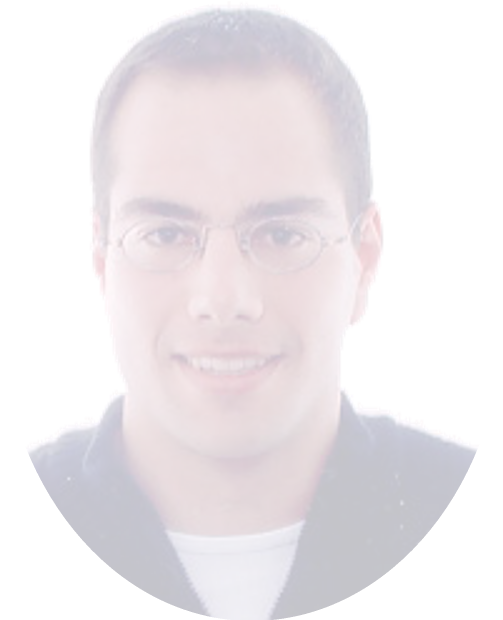
\includegraphics{hofert.png}}

\newtcbtheorem[number within=section]{mythm}{Theorem}%
{colback=green!5,colframe=green!35!black,fonttitle=\bfseries,breakable}{th}
\newtcbtheorem[use counter from=mythm]{mydef}{Definition}%
{colback=blue!5,colframe=blue!35!black,fonttitle=\bfseries,breakable}{de}
\newtcbtheorem[use counter from=mythm]{myrem}{Remark}%
{colback=white!5,colframe=white!35!black,fonttitle=\bfseries,breakable}{re}
\newtcbtheorem[use counter from=mythm]{myex}{Example}%
{colback=orange!5,colframe=orange!35!black,fonttitle=\bfseries,breakable}{ex}
\newtcbtheorem[use counter from=mythm]{myprop}{Proposition}%
{colback=green!5,colframe=green!35!black,fonttitle=\bfseries,breakable}{pr}

\setcounter{tocdepth}{2}
\setlength\parindent{0pt}
\hyphenpenalty 10000

\title{STAT 240 Course Notes - Fall 2018}
\author{Max Zhu}

\begin{document}
	\maketitle
	\tableofcontents\newpage
	
	\section{Foundations}
	Andrey Kolmogorov \textit{(1933, ``Foundations of the theory of probability")} put probability on solid mathematical grounds using a model, probability space $(\Omega, \mathcal{F}, P)$. A probability space consists of:
	\begin{enumerate}
		\item Sample space $\Omega$: set of all outcomes $\omega$
		\item $\sigma$-algebra $\mathcal{F}$: set of all events, i.e. subsets of $\Omega$ to which we can assign a probability
		\item Probability measure $P: \mathcal{F} \rightarrow  [0, 1]$: function which assigns probabilities to events
	\end{enumerate}
	
	We need measure theory to understand this.
	
	\subsection{$\sigma$-algebras and measures}
	A classical problem is to measure the volume $\lambda(A)$ of some $A\subseteq \mathbb{R}^d, d\geq 1$. Consider $d=1$. Then, $\lambda$ should:
	\begin{enumerate}[label=(\roman*)]
		\item Assign to intervals its length: $\lambda([a, b])=b-a$ for all $a, b\in \mathbb{R}, a \leq b$
		\item Be invariant under translations, rotations, and reflections: $\lambda(A)=\lambda(B)$ for all congruent $A, B\subseteq \mathbb{R}$
		\item Be $\sigma$-additive:\\
		If $\{A_i\}_{i\in\mathbb{N}}\subseteq\mathbb{R}, A_i\cap A_j=\varnothing\;\forall i\neq j$, then $\lambda(\bigcup_{i=1}^{\infty}A_i)=\sum_{i=1}^{\infty}\lambda(A_i)$\\\\
		In other words, the volume of the union of countably many subsets of $\mathbb{R}$ is equal to the sum of their volumes.
	\end{enumerate}
	
	Can we take the power set $\mathcal{P}(\mathbb{R})=\{A : A\subseteq \mathbb{R}\}$ as $\mathcal{F}$ and find such a $\lambda$?
	
	\begin{mythm}{Vitali's Theorem}{}
		There exists no $\lambda$ defined on $\mathcal{P}(\mathbb{R})$ which fulfils (i)-(iii). Furthermore, any measurable set $A\subseteq\mathbb{R}: \lambda(A)>0$ contains a non-measurable set $V$ (Vitali set). 
	\end{mythm}
	
	What about weakening (iii) to finitely many sets? Still no!
	
	\begin{mythm}{Banach-Tarski}{}
		Let $d\geq 3$ and $A, B\in \mathbb{R}^d$ be bounded with non-empty interior. Then, there exists $k\in\mathbb{N}$ and partitions:
		\begin{align*}
			A=\dot\bigcup_{i=1}^kA_i\\
			B=\dot\bigcup_{i=1}^kB_i
		\end{align*}
		such that $A_i, B_i$ are congruent $\forall i\in \{1,\dots, k\}$.
	\end{mythm}
	
	For countable $\Omega$, one can define $\lambda$ (or $\mu$ or $P$) on $\mathcal{P}(\Omega)$ but for uncountable $\Omega$, $\mathcal{P}(\Omega)$ is too large. Therefore, we need to define $\lambda, \mu,$ or  $P$ on some proper subset of $\mathcal{P}(\Omega)$ which is closed under certain set operations.
	
	\begin{mydef}{$\sigma$-algebra}{}
		$\mathcal{F}\subseteq\mathcal{P}(\Omega)$ is a \underline{$\sigma$-algebra} on $\Omega$ if:
		\begin{enumerate}[label=(\roman*)]
			\item $\Omega\in\mathcal{F}$
			\item $A\in\mathcal{F}\Rightarrow A^c\in\mathcal{F}$
			\item $\{A_i\}_{i\in\mathbb{N}}\subseteq\mathcal{F}\Rightarrow\bigcup_{i=1}^{\infty}A_i\in\mathcal{F}$
		\end{enumerate}
		If (iii) holds for only finitely many sets, $\mathcal{F}$ is an \underline{algebra}.
	\end{mydef}
	
	\begin{myrem}{}{}
		$\sigma$-algebras are closed w.r.t. countable intersection, since
		\begin{equation*}
			\bigcap_{i=1}^{\infty}A_i=(\bigcup_{i=1}^{\infty}A_i^c)^c\in\mathcal{F}
		\end{equation*}
		by de Morgan.
	\end{myrem}
	
	\begin{myex}{}{}
		\begin{enumerate}
			\item Trivial $\sigma$-algebra: $\{\varnothing, \Omega\}=\mathcal{F}$
			\item $\mathcal{F}=\{\dot\bigcup_{i=1}^n(a_i, b_i] : 0\leq a_i\leq b_i\leq 1\;\forall i, n\in\mathbb{N}\}$ is an algebra on $\Omega=(0, 1]$ but not a $\sigma$-algebra since $\dot\bigcup_{n=0}^{\infty}(\sum_{k=1}^{2n}(\frac{1}{2})^k, \sum_{k=1}^{2n+1}(\frac{1}{2})^k]\notin\mathcal{F}$, while $(\sum_{k=1}^{2n}(\frac{1}{2})^k, \sum_{k=1}^{2n+1}(\frac{1}{2})^k]\in\mathcal{F}$ for all $k$.
		\end{enumerate}
	\end{myex}
	
	How can $\sigma$-algebras be constructed?
	
	\begin{myprop}{}{}
		Given $A\subseteq\mathcal{P}(\Omega)$, then there exists a unique minimal $\sigma$-algebra $\sigma(A)$ which contains all sets of $A$: a $\sigma$-algebra generated by A. $\sigma(A)$ is the intersection of all $\sigma$-algebras of which A is a subset.
		
		\begin{proof}
		Let $\mathcal{F}_A=\{\mathcal{F} : \mathcal{F}$ is a $\sigma$-algebra, $A\subseteq\mathcal{F}\}$. Then, $\sigma(A)$ is a $\sigma$-algebra since:
		\begin{enumerate}[label=(\roman*)]
			\item $\Omega\in\mathcal{F}\;\forall\mathcal{F}\in\mathcal{F}_A$ since all $\mathcal{F}\in\mathcal{F}_a$ is a $\sigma$-algebra
			\item $A\in\sigma(A)\Rightarrow A\in\mathcal{F}\;\forall\mathcal{F}\in\mathcal{F}_A\Rightarrow A^c\in\mathcal{F}\;\forall\mathcal{F}\in\mathcal{F}_A\Rightarrow A^c\in\sigma(A)$.
			\item If $\{A_i\}_{i\in\mathbb{N}}\subseteq \sigma(A)$, then $\{A_i\}_{i\in\mathbb{N}}\subseteq\mathcal{F}\;\forall\mathcal{F}\in\mathcal{F}_A$.\\ So, $\bigcup_{i=1}^{\infty}A_i\in\mathcal{F}\;\forall\mathcal{F}\in\mathcal{F}_A$, so $\bigcup_{i=1}^{\infty}A_i\in\sigma(A)$.
		\end{enumerate}
		
		So $\sigma(A)$ is a $\sigma$-algebra. Now, $\sigma(A)\supseteq A$ since $\mathcal{F}\supseteq A\;\forall\mathcal{F}\in\mathcal{F}_A$. Also, $\forall\;\sigma$-algebra $\mathcal{F}'\supset A$, we have $\mathcal{F}'\in\mathcal{F}_A$, so $\mathcal{F}'\supseteq\sigma(A)$.\\
		
		Therefore, $\sigma(A)$ is the minimal $\sigma$-algebra containing A.
	\end{proof}
	\end{myprop}
	
	\begin{myrem}{}{}
		Unless $|\Omega|<\infty$, a construction of $\sigma(A)$ is typically hopeless.
	\end{myrem}
	
	\begin{myex}{}{}
		$\mathcal{B}(\Omega):=\sigma(\{O : O\subseteq\Omega, O$ is open$\})$ is the Borel $\sigma$-algebra on $\Omega$. Its elements are called Borel sets. For $\Omega=\mathbb{R}^d$ one can show that
		\begin{align*}
			\mathcal{B}(\mathbb{R}^d)&=\sigma(\{(a, b] : a\leq b\})\\
			&=\sigma(\{(a, b) : a\leq b\})\\
			&=\sigma(\{[a, b] : a\leq b\})\\
			&=\sigma(\{(-\infty, b]\})
		\end{align*}
		and so on. Borel sets contain open sets, closed sets, and countable union and intersections of these sets.
	\end{myex}
	
	\begin{mydef}{Measure Space}{}
			Let $\mathcal{F}$ be a $\sigma$-algebra on $\Omega$. Then, $(\Omega, \mathcal{F})$ is a \underline{measurable space}, sets in $\mathcal{F}$ are \underline{measurable sets}. A \underline{measure} $\mu$ on $\mathcal{F}$ is a function such that:
			\begin{enumerate}[label=(\roman*)]
				\item $\mu : \mathcal{F}\rightarrow [0, \infty]$
				\item $\mu(\varnothing)=0$
				\item Let $\{A_i\}_{i\in\mathbb{N}}\subseteq\mathcal{F}, A_i\cap A_j=\varnothing\;\forall i\neq j$. Then, $\mu(\dot\bigcup_{i=1}^{\infty}A_i)=\sum_{i=1}^{\infty}\mu(A_i)$. ($\sigma$-additivity)
			\end{enumerate}
			
			$(\Omega, \mathcal{F}, \mu)$ is then called a \underline{measure space}.\\
			
			If $\Omega=\bigcup_{i=1}^{\infty}A_i$ for $\{A_i\}_{i\in\mathbb{N}}\subseteq\mathcal{F}: \mu(A_i)<\infty\;\forall i$, then $\mu$ is \underline{$\sigma$-finite}.\\
			
			If $\mu(\Omega)<\infty$, $\mu$ is a \underline{finite measure}.\\
			
			A measure $\mu$ on $\mathcal{B}(\mathbb{R}^d)$ is a \underline{Borel measure} on $\mathbb{R}^d$.
	\end{mydef}
	
	\begin{myrem}{}{}
		\begin{enumerate}
			\item $\sigma$-additivity (in contrast to finite additivity) allows for limiting processes (pointwise limits of "measurable functions" are measurable). Many fundamental consequences follow, such as Central Limit Theorem and Law of Large Numbers.
			\item Uncountable additivity is too strong, since for any $A\subseteq \mathbb{R}$:
			\begin{align*}
				\lambda(A)&=\lambda(\bigcup_{x\in A}\{x\})\\
				&=\sum_{x\in A}\lambda(\{x\})\\
				&=sup_{A'\subseteq A, |A'|<\infty}\sum_{x\in A}\lambda(\{x\})\\
				&=0
			\end{align*}
		\end{enumerate}
	\end{myrem}
	
	\begin{myex}{}{}
		If $\Omega$ is countable, $\mathcal{F}=\mathcal{P}(\Omega)$, $\forall f : \Omega\rightarrow[0, \infty]$, $\mu(A)=\sum_{\omega\in A}f(\omega)\;\forall A\in\mathcal{F}$ defines a measure on $\mathcal{F}$.\\
		
		If $f(x)=1\;\forall x\in\Omega$, $\mu$ is called a counting measure.\\
		
		Suppose for some $\omega_0\in\Omega, f(\omega)=1$ if $\omega=\omega_0$, $0$ otherwise. Then $\mu$ is point mass or Dirac measure.
	\end{myex}
	
	\begin{myprop}{}{}
		Let $(\Omega, \mathcal{F}, \mu)$ be a measure space. Then:
		\begin{enumerate}
			\item $A, B\in\mathcal{F}, A\subseteq B\Rightarrow\mu(\bigcup_{i=1}^{\infty}A_i)\leq\sum_{i=1}^{\infty}\mu(A_i)$ (monotonicity)
			\item $\{A_i\}_{i\in\mathbb{N}}\subseteq\mathcal{F}\Rightarrow\mu(\bigcup_{i=1}^{\infty}A_i)\leq\sum_{i=1}^{\infty}\mu(A_i)$ (sub additivity)
			\item \begin{align*}
				\{A_i\}_{i\in\mathbb{N}}\subseteq\mathcal{F}, A_1\subseteq\dots\subseteq A_n\subseteq\dots\Rightarrow\mu(\bigcup_{i=1}^{\infty}A_i)&=\mu(\lim_{n\to\infty}\bigcup_{i=1}^{n}A_i)\\
				&=\lim_{n\to\infty}\mu(A_n)
			\end{align*}
			(continuity from below)
			\item \begin{align*}
				\{A_i\}_{i\in\mathbb{N}}\subseteq\mathcal{F}, A_1\supseteq\dots\supseteq A_n\supseteq\dots\Rightarrow\mu(\bigcap_{i=1}^{\infty}A_i)&=\mu(\lim_{n\to\infty}\bigcap_{i=1}^{n}A_i)\\
				&=\lim_{n\to\infty}\mu(A_n)
			\end{align*} for $\mu(A_1)<\infty$.
			(continuity from above)
		\end{enumerate}
		
		\begin{proof}~\\
		\begin{enumerate}
			\item $B=A\dot\cup(B\backslash A)$\\
			Therefore, $\mu(B)=\mu(A)+\mu(B\backslash A)\geq0$\\
			$\mu(B)\geq\mu(A)$ and if $\mu(A)<\infty$,\\
			$\mu(B\backslash A)=\mu(B)-\mu(A)$.
			\item Let $B_1=A_1$, $B_n=A_n\backslash \bigcup_{i=1}^{n-1}A_i\subseteq A_n\;\forall n\geq2$.\\
			So, all $B_n$ are pairwise disjoint and $\bigcup_{i=1}^{n}B_i=\bigcup_{i=1}^{n}A_i\;\forall n\in\mathbb{N}$.\\
			So, $\mu(\bigcup_{i=1}^{\infty}A_i)=\mu(\bigcup_{i=1}^{\infty}B_i)=\sum_{i=1}^{\infty}\mu(B_i)\leq\sum_{i=1}^{\infty}\mu(A_i)$.
			\item Let $A_0=\varnothing$. Then,
			\begin{align*}
				\mu(\bigcup_{i=1}^{\infty}A_i)&=\mu(\bigcup_{i=1}^{\infty}(A_i\backslash A_{i-1})\\
				&=\sum_{i=1}^{\infty}\mu(A_i\backslash A_{i-1})\\
				&=\lim_{n\to\infty}\sum_{i=1}^{n}\mu(A_i\backslash A_{i-1})\\
				&=\lim_{n\to\infty}\mu(A_n)
			\end{align*}
			\item Let $B_i=A_1\backslash A_i=A_1\cap A_i^c\;\forall i\in\mathbb{N}$. Then, $B_1\subseteq B_2\subseteq\dots$
			\begin{align*}
				\bigcup_{i=1}^{\infty}B_i&=\bigcup_{i=1}^{\infty}(A_1\cap A_i^c)\\
				&=A_1\cap\bigcup_{i=1}^{\infty}A_i^c\\
				&=A_1\cap(\bigcap_{i=1}^{\infty}A_i)^c\\
				&=A_1\backslash\bigcap_{i=1}^{\infty}A_i\Rightarrow\\
				\mu(A_i)-\mu(\bigcap_{i=1}^{\infty}&=\mu(A_1\backslash\bigcap_{i=1}^{\infty}A_i)\\
				&=\mu(\bigcup_{i=1}^{\infty}B_i)\\
				&=\lim{n\to\infty}\mu(B_n)\\
				&=\lim_{n\to\infty}(\mu(A_1)-\mu(A_n))\\
				&=\mu(A_1)-\lim_{n\to\infty}\mu(A_n)\\
				\therefore\mu(\bigcap_{i=1}^{\infty}&=\lim_{n\to\infty}\mu(A_n)
			\end{align*}
			
		\end{enumerate}
	\end{proof}
	\end{myprop}
	
	\newpage\subsection{Probability Measures}
	
	\begin{mydef}{Probability Measure}{}
		Let $(\Omega, \mathcal{F})$ be a measure space. Then, a \underline{probability measure} $P$ on $\mathcal{F}$ is a function such that:
		\begin{enumerate}[label=(\roman*)]
			\item $P : \mathcal{F}\to[0, 1]$
			\item $P(\Omega)=1$
			\item $\{A_i\}_{i\in\mathbb{N}}\subseteq\mathcal{F}, A_i\cap A_j=\varnothing\;\forall i\neq j\Rightarrow P(\dot\bigcup_{i=1}^{\infty}A_i)=\sum_{i=1}^{\infty}(A_i)$\\($\sigma$-additivity)
		\end{enumerate}
		
		$(\Omega, \mathcal{F}, P)$ is a \underline{probability space}.\\
		
		$\Omega$ is a \underline{sample space}.\\
		
		$\omega\in\Omega$ is a \underline{sample point}.\\
		
		If $\Omega$ is countable/finite, then $(\Omega, \mathcal{F}, P)$ is \underline{discrete/finite}.\\
		
		Any $A\in\mathcal{F}$ is an \underline{event}.\\
		
		If $A=\{\omega\}$, A is a \underline{simple event}.\\
		
		Otherwise, A is a \underline{compound event}.\\
	\end{mydef}
	
	\begin{myrem}{}{}
		If $(\Omega, \mathcal{F}, P)$ is discrete, $f(\omega):=P(\{\omega\}), \omega\in\Omega$ defines $P$ via $P(A)=\sum_{\omega\in A}f(\omega), A\in\mathcal{F}$. Then, $f$ is the probability mass function (pmf) on $\Omega$.\\
		
		Conversely, if $\Omega$ is countable, then in $(\Omega, \mathcal{P}(\Omega), P)$ with $P(A):=\sum_{\omega\in A}f(\omega)$, $A\in\mathcal{P}(\Omega)$, $P$ defines a discrete probability measure for any $f : \Omega\to[0, 1]$ such that $\sum_{\omega\in A}f(\omega)=1$.
	\end{myrem}
	
	\begin{myprop}{}{}
		Let $(\Omega, \mathcal{F}, P)$ be a probability space. Then,
		\begin{enumerate}
			\item $A\in\mathcal{F}\Rightarrow P(A^c)=1-P(A)$
			\item $A, B\in\mathcal{F}\Rightarrow P(A\cup B)=P(A)+P(B)-P(A\cap B)$
			\item Let $\{A_i\}_{i\in\mathbb{N}}\subseteq\mathcal{F}$\\
			$S_{k, n}:=\sum_{1\leq i_1<\dots<i_k\leq n}P(A_{i_1}\cap\dots\cap A_{i_k})$, for $k=1,\dots,n$\\
			
			Then, $P(\bigcup_{i=1}^{n}A_i)=\sum_{i=1}^{n}(-1)^{k-1}S_{k, n}$\\
			
			(inclusion-exclusion principle)
		\end{enumerate}
		
		\begin{proof}~\\
		\begin{enumerate}
			\item $1=P(\Omega)=P(A\dot\cup A^c)=P(A)+P(A^c)$\\
			
			This implies probability measures are measures (take $A=\varnothing$).
			\item $A\cup B=(A\backslash(A\cap B))\dot\cup(A\cap B)\dot\cup(B\backslash(A\cap B))\Rightarrow$
			\begin{align*}
				P(A\cup B)&=P(A)-P(A\cap B)+P(A\cap B)+P(B)-P(A\cap B)\\
				&=P(A)+P(B)-P(A\cap B)
			\end{align*}
			\item Induction on n. See Exercise 6 in Assignment 1.
		\end{enumerate}
	\end{proof}
	\end{myprop}
	
	\newpage\subsection{Null Sets}	
	
	\begin{mydef}{Null Set}{}
		If $(\Omega, \mathcal{F}, \mu)$ is a measure space, every $N\in\mathcal{F}$ such that $\mu(N)=0$ is a \underline{($\mu$-)null set}.\\
		
		If some property holds $\forall\omega\in\Omega\backslash N$ for null set $N$, it holds \underline{($\mu$-)almost everywhere}.\\
		
		Or, if $\mu$ is a probability measure, \underline{($\mu$-)almost surely}.\\
		
		If $\mathcal{F}$ contains all subsets of null sets, $\mu$ is \underline{complete}.
	\end{mydef}
	
	By sub additivity, any countable union of null sets from $\mathcal{F}$ is a null set of $\mathcal{F}$.
	
	\begin{mythm}{Completion}{comp}
	Let $(\Omega, \mathcal{F}, \mu)$ be a measure space, $\mathcal{N}$ be the set of all null sets.
		\begin{enumerate}
			\item $\bar{\mathcal{F}}:=\{F\cup A : F\in\mathcal{F}, A\subseteq N, N\in\mathcal{N}\}$ is a $\sigma$-algebra on $\Omega$.
			\item $\bar{\mu}(F\cup A)=\mu(F)$ uniquely extends $\mu$ to a complete measure on $\bar{\mathcal{F}}$.
		\end{enumerate}
	\end{mythm}
	
	\newpage\subsection{Construction of Measures}
	
	Idea: Functions with properties as measures (premeasures) defined on a ring can be extended
to complete measures on the $\sigma$-algebra generated by the ring.

	\begin{mydef}{Rings}{}
		$\mathcal{R}\subseteq\mathcal{P}(\Omega)$ is a \underline{ring} on $\Omega$ if:
		\begin{enumerate}
			\item $\varnothing\in\mathcal{R}$
			\item $A, B\in\mathcal{R}\Rightarrow A\backslash B\in\mathcal{R}$
			\item $A, B\in\mathcal{R}\Rightarrow A\cup B\in\mathcal{R}$
		\end{enumerate}
		
		A \underline{premeasure} $\mu_0$ on $\mathcal{R}$ is a function with:
		\begin{enumerate}[label=(\roman*)]
			\item $\mu_0 : \mathcal{R}\to[0, \infty]$
			\item $\mu_0(\varnothing)=0$
			\item $\{A_i\}_{i\in\mathbb{N}}\subseteq\mathcal{R}, A_i\cap A_j=\varnothing\;\forall i\neq j, \dot\bigcup_{i=1}^{\infty}A_i\in\mathcal{R}\Rightarrow\mu(\dot\bigcup_{i=1}^{\infty}A_i)=\sum_{i=1}^{\infty}\mu_0(A_i)$
		\end{enumerate}
	\end{mydef}
	
	\begin{mythm}{Caratheodory's extension theorem}{cara}
		If $\mu_0$ is a premeasure on ring $\mathcal{R}$ on $\Omega$, there exists a complete measure $\mu$ on $\mathcal{F}:=\sigma(\mathcal{R})$ which coincides with $\mu_0$ on $\mathcal{R}$. If $\mu_0$ is $\sigma$-finite, then $\mu$ is unique.
	\end{mythm}
	
	\begin{myrem}{}{}
		The proof of \ref{th:cara} is constructive. The measure $\mu$ is constructed:
		\begin{align*}
			\mu(A)&=\inf_{A\subseteq\bigcup_{i=1}^{\infty}A_i, A_i\in\mathcal{R}\;\forall i}\sum_{i=1}^{\infty}\mu_0(A_i)\\
			&=A_i\in\mathcal{R}\;\forall i
		\end{align*}
	\end{myrem}
	
	\begin{mythm}{}{righ}
		If $F : \mathbb{R}\to\mathbb{R}$ is right-continuous and increasing ($F(x)\leq F(y)\;\forall x<y$), there exists exactly one Borel measure $\mu_F$ such that:\\
		
		$\mu_F((a, b])=F(b)-F(a)\;\forall a\leq b$
		
		\begin{proof}
			$\mathcal{R}:=\{\dot\bigcup_{k=1}^{n}(a_k, b_k] : -\infty<a_k\leq b_k<\infty\;\forall k, n\in\mathbb{N}\}$ is a ring on $\mathbb{R}$, and $\mu_0(\dot\bigcup_{k=1}^{n}(a_k, b_k]):=\sum_{k=1}^{n}(F(b_k)-F(a_k))$ is a premeasure on $\mathcal{R}$. By \ref{th:cara}, there exists exactly one measure $\mu_F$ on $\sigma(\mathbb{R})=\mathcal{B}(\mathbb{R})$ such that $\mu_F|_{\mathcal{R}}=\mu_0$ (i.e. $\mu_F(A)=\mu_0(A)\;\forall A\in\mathbb{R}$).
		\end{proof}
	\end{mythm}
	
	\begin{myrem}{}{}
		\begin{enumerate}
			\item By \ref{th:cara}, $\mu_F$ is complete, and called the Lebesgue-Stietjes measures associated to $F$. Its domain, the completion $\bar{\mathcal{B}}(\mathbb{R})$, the Lebesgue $\sigma$-algebra, can be shown to strictly contain $\mathcal{B}(\mathbb{R})$. Sets in $\bar{\mathcal{B}}(\mathbb{R}$ are called Lebesgue measurable or Lebesgue sets. By our construction,
			\begin{equation*}
				\mu_F(A)=\inf_{A\subseteq\bigcup_{i=1}^{\infty}(a_i, b_i]}\sum_{i=1}^{\infty}\mu_F((a, b])
			\end{equation*}
			\item If $F(x)=x$, $\lambda:=\mu_F$ is a Lebesgue measure on $\mathbb{R}$. Sets $N\subseteq\bar{\mathcal{B}}(\mathbb{R})$ that are null sets are Lebesgue null sets, $\lambda(N)=0$.\\
			
			By \ref{th:comp} (1), $B\in\bar{\mathcal{B}}(\mathbb{R})\Leftrightarrow B=A\cup N$.
		\end{enumerate}
	\end{myrem}
	
	\begin{myex}{}{}
		\begin{enumerate}
			\item $\{x\}\subseteq\mathbb{R}$ is a null set for all $x\in\mathbb{R}$, since
			\begin{align*}
				\lambda(\{x\})&=\lambda\big(\bigcap_{n=1}^{\infty}(x-\frac{1}{n}, x]\big)\\
				&=\lim_{n\to\infty}\lambda\big((x-\frac{1}{n}, x]\big)\\
				&=0
			\end{align*}
			\item $\mathbb{Q}\subseteq\mathbb{R}$ is a null set since
			\begin{align*}
				\lambda(\mathbb{Q})&=\lambda(\dot\bigcup_{i=1}^{\infty}\{q_i\})\\
				&=\sum_{i=1}^{\infty}0\\
				&=0
			\end{align*}
			\item Cantor set: $C=\bigcap_{i=1}^{\infty}C_i$ where $C_i$ is defined by:
			\begin{align*}
				C_0&=[0,1]\\
				C_1&=[0,\frac{1}{3}]\cup[\frac{2}{3}, 1]\\
				C_2&=[0,\frac{1}{9}]\cup[\frac{2}{9}, \frac{1}{3}]\cup[\frac{2}{3}, \frac{7}{9}]\cup[\frac{8}{9}, 1]\\
				\dots\\
				C_i&=\frac{C_{i-1}}{3}\cup(\frac{2}{3}+\frac{C_{i-1}}{3})\;\forall i\geq1
			\end{align*}
			
			By Cantor's diagonal argument, C is uncountable. Since $\lambda([0, 1]\backslash C)=2^0\frac{1}{3}+2^1\frac{1}{9}+\dots=\sum_{i=1}^{\infty}2^{i-1}3^{-i}=1$, therefore $\lambda(C)=0$.
		\end{enumerate}
	\end{myex}
	
	\begin{myrem}{}{}
		\ref{th:righ} extends to $F : \mathbb{R}^d\to\mathbb{R}$ which is:
		\begin{enumerate}[label=(\roman*)]
			\item right continuous: $F(\underline{x})=\lim_{\underline{h}\downarrow\underline{0}}F(\underline{x}+\underline{h})=:F(\underline{x}+)\;\forall x\in\mathbb{R}^d$
			\item d-increasing: The F-volume $\Delta_{(\underline{a}, \underline{b}]}F$ of $(a, b]\geq0$ for $\underline{a}\leq\underline{b}$, where:
			\begin{align*}
				\Delta_{(\underline{a}, \underline{b}]}F:&=\sum_{i\in\{0, 1\}^d}(-1)^{\sum_{j=1}^{d}ij}F(a_1^{i_1}b_1^{1-i_1}, \dots, a_d^{i_d}b_d^{1-i_d})\\
				&=\prod_{j=1}^{d}(b_j-a_j)\\
				&=\lambda((a, b])
			\end{align*}
			\item If, additionally, $\lim_{x_j\downarrow-\infty}F(\underline{x})=0$ for some $j\in\{1, \dots, d\}$ and $F(\underline{\infty})=lim_{\underline{x}\uparrow\infty}F(x)=1$, then $\mu_F$ is a probability measure on $\mathcal{B}(\mathbb{R}^d)$. Then, $\Delta_{(a, b]}F$ is the probability of $(\underline{a}, \underline{b}]$.
		\end{enumerate}
	\end{myrem}
	
	\newpage
	\section{Geometric and Laplace probability spaces}
	
	\begin{myprop}{}{prob}
		Let $(\Omega, \mathcal{F}, \mu)$ be a measure space such that $0<\mu(\Omega)<\infty$. Then, $(\Omega, \mathcal{F}, P)$ with $P(A)=\frac{\mu(A)}{\mu(\Omega}\;\forall A\in\mathcal{F}$, is a probability space. 
		
		\begin{proof}~\\
			\begin{enumerate}[label=(\roman*)]
				\item $0\leq\mu(A)\leq\mu(\Omega)\leq\infty\;\forall A\in\mathcal{F}\Rightarrow P : \mathcal{F}\to[0, 1]$
				\item $P(\Omega)=\frac{P(\Omega)}{P(\Omega)}=1$
				\item $\{A_i\}_{i\in\mathbb{N}}\subseteq\mathcal{F}, A_i\cap A_j=\varnothing\;\forall i\neq j\Rightarrow$
				\begin{align*}
					P(\bigcup_{i=1}^{\infty}A_i)&=\frac{\mu(\bigcup_{i=1}^{\infty}A_i)}{\mu(\Omega}\\
					&=\sum_{i=1}^{\infty}\frac{\mu(A_i)}{\mu(\Omega}\\
					&=\sum_{i=1}^{\infty}P(A_i)
				\end{align*}
			\end{enumerate}
		\end{proof}
	\end{myprop}
	
	If $\mathcal{F}$ is a $\sigma$-algebra on $\Omega$ and $\Omega'\subseteq\Omega$, one can show that the restriction\\
	$\mathcal{F}|_{\Omega'}:=\{A\cap\Omega' : A\in\mathcal{F}\}$ is a $\sigma$-algebra on $\Omega'$. This is called the trace $\sigma$-algebra of $\Omega'$ in $\mathcal{F}$.
	
	\newpage\subsection{Geometric Probability Spaces}
	\begin{mydef}{Geometric Probability Space}{}
		If:
		\begin{align*}
			\Omega&\subseteq\mathbb{R}^d : 0<\lambda(\Omega)<\infty\\
			\mathcal{F}&=\mathcal{B}(\Omega) \\
			P(A)&=\frac{\lambda(A)}{\lambda(\Omega)}\;\forall A\in\mathcal{F}
		\end{align*}
		then the probability space $(\Omega, \mathcal{F}, P)$ is a \underline{geometric probability space}.
	\end{mydef}
	
	\begin{myex}{}{}
		A stick length $l$ is randomly marked and cut at 2 spots. Find the probability that the 3 pieces can form a triangle.
		
		\paragraph{Solution.}
		Let
		\begin{align*}
			\Omega&=\{(\omega_1, \omega_2)\in[0, l]^2, \omega_1<\omega_2\}\\
			\mathcal{F}&=\bar{\mathcal{B}}(\Omega)\\
			P(A)&=\frac{\lambda(A)}{\lambda(\Omega)}
		\end{align*}
		
		We are interested in the set A: ``each side \textless\; sum of other 2", or
		\begin{align*}
			A=&\{(\omega_1, \omega_2)\in\Omega :\\
			&\omega_1<(\omega_2-\omega_1)+(l-\omega_2),\\
			&\omega_2-\omega_1<\omega_1+l-\omega_2,\\
			&l-\omega_2<\omega_1+\omega_2-\omega_1\}\\
			=&\{(\omega_1, \omega_2)\in\Omega : \omega_1<\frac{l}{2}, \frac{l}{2}<\omega_2<\omega_1+\frac{l}{2}\}
		\end{align*}
		
		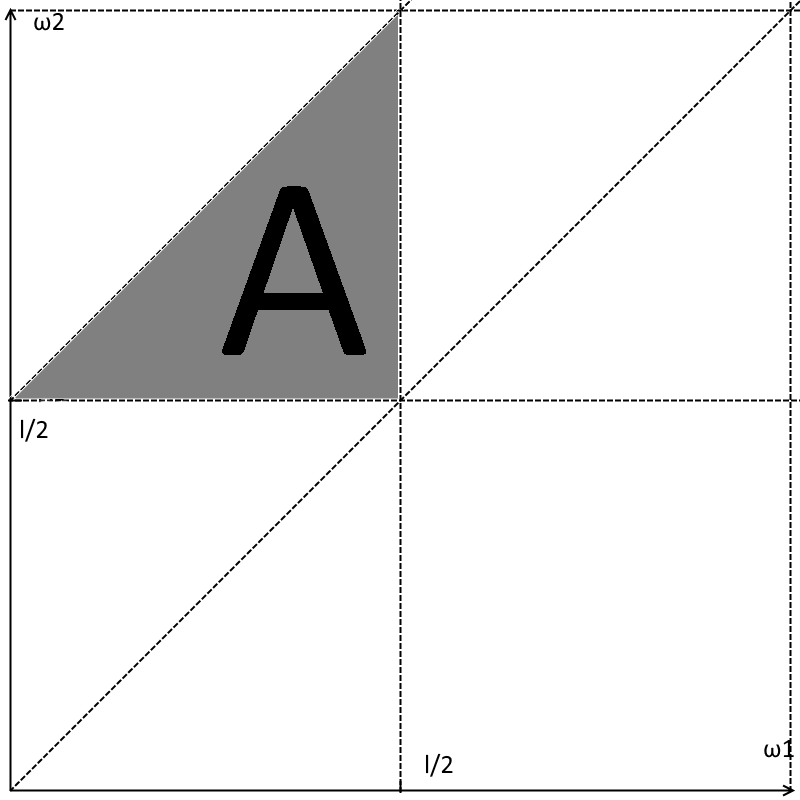
\includegraphics[width=100pt]{triangle.png}
		
		$P(A)=\frac{1}{4}$, from the picture.
	\end{myex}
	
	\newpage\subsection{Laplace Probability Spaces}
	Here is a similar construction, based on the number $|\Omega|$ of elements in $\Omega$.
	\begin{myprop}{}{}
		Let $1\leq|\Omega|<\infty$, $\mathcal{F}=\mathcal{P}(A), P(A)=\frac{|A|}{|\Omega|}\;\forall A\in\mathcal{F}$. Then, $(\Omega, \mathcal{F}, P)$ is a finite probability space called a Laplace probability space.\\
		
		$P$ is discrete uniform distribution on $\Omega$.
		
		\begin{proof}
			Apply Prop. \ref{pr:prob} with $\mu(A)=|A|$ (counting measure).
		\end{proof}
	\end{myprop}
	
	\begin{myrem}{}{}
		For Laplace probability spaces, probability mass function on $\Omega$ is\\
		
		$f(\omega)=P(\{\omega\})=\frac{|\{\omega\}|}{|\Omega|}=\frac{1}{|\Omega|}\;\forall\omega\in\Omega$
		
		so the discrete uniform distribution assigns equal probability $\frac{1}{|\Omega|}$ to each $\omega\in\Omega$.
	\end{myrem}
	
	\begin{myex}{}{}
		\begin{enumerate}
			\item Determine probability of obtaining 1 or 5 when rolling a fair, 6-sided die.
			\begin{align*}
				\Omega&=\{1, \dots, 6\}\\
				\mathcal{F}&=\mathcal{P}(\Omega)\\
				P(A)&=\frac{|A|}{|\Omega|}\;\forall A\in\Omega
			\end{align*}
			
			Let $A=$``rolling 1 or 5"$=\{1, 5\}$. Then, $P(A)=\frac{2}{6}=\frac{1}{3}$.
			\item Determine probability of obtaining a sum of 2 and 7 when rolling the die twice.
			\begin{align*}
				\Omega&=\begin{matrix}
				\{(1, 1), & \dots, & (1, 6),\\
				& \ddots & \\
				(6, 1), & \dots, & (6, 6)\}
				\end{matrix}\\
				\mathcal{F}&=\mathcal{P}(\Omega)\\
				P(A)&=\frac{|A|}{|\Omega|}\;\forall A\in\mathcal{F}
			\end{align*}
			
			So,\\
			
			$P($``sum is 2"$)=\frac{1}{36}$\\
			
			$P($``sum is 7"$)=\frac{6}{36}=\frac{1}{6}$\\
			\item Determine probability of obtaining at least one 6 when rolling 3 times.
			\begin{align*}
				\Omega&=\{(\omega_1, \omega_2, \omega_3) | \omega_i\in\{1, \dots, 6\}\;\forall i\}\\
				\mathcal{F}&=\mathcal{P}(\Omega)\\
				P(A)&=\frac{|A|}{|\Omega|}\;\forall A\in\mathcal{F}
			\end{align*}
			
			So, $P($``at least one 6"$)=1-P($``no 6s"$)=1-(\frac{5}{6})^3=\frac{91}{216}$
		\end{enumerate}
	\end{myex}
	
	\newpage
	\section{Probability Counting Techniques}
	\subsection{Basic Rules}
	
	\begin{myprop}{}{}
		\begin{enumerate}
			\item If $A_1, \dots, A_n$ are pointwise disjoint finite sets, then\\
			$|\bigcup_{i=1}^{n}A_i|=\sum_{i=1}^{n}|A_i|$ (addition rule).
			\item If $A_1, \dots, A_n$ are finite sets, then\\
			$|\prod_{i=1}^{n}A_i|=\prod_{i=1}^{n}|A_i|$ (multiplication rule).
		\end{enumerate}
		
		\begin{proof}
			By induction.
		\end{proof}
	\end{myprop}
	
	\begin{myex}{}{}
		Consider an urn with 5 balls labelled 1, \dots, 5. Determine the probability of obtaining precisely 1 even ball when drawing twice with replacement. Let $\mathbb{E}$ be the set of even integers.
		\begin{align*}
			\Omega&=\begin{matrix}
				\{(1, 1), & \dots, & (1, 5),\\
				& \ddots & \\
				(5, 1), & \dots, & (5, 5)\}
				\end{matrix}\\
			\mathcal{F}&=\mathcal{P}(\Omega)\\
			A&=\{(\omega_1, \omega_2)\in\Omega : \omega_1+\omega_2\notin\mathbb{E}\}\\
			&=A_1\dot\cup A_2
		\end{align*}
		where
		\begin{align*}
			A_1&=\{(\omega_1, \omega_2) : \omega_1\in\mathbb{E}, \omega_2\notin\mathbb{E}\}\\
			A_2&=\{(\omega_1, \omega_2) : \omega_1\notin\mathbb{E}, \omega_2\in\mathbb{E}\}\\
			\therefore P(A)&=\frac{|A|}{|\Omega|}\\
			&=\frac{|A_1|+|A_2|}{|\Omega|}\\
			&=\frac{2*3+3*2}{25}\\
			&=\frac{12}{25}
		\end{align*}
	\end{myex}
	
	\subsection{Urn Models}
	Many counting problems can be associated with drawing k balls from an urn with n balls. Classical models consider drawing:
	\begin{enumerate}[label=(\Roman*)]
		\item With order, with replacement
		\item With order, without replacement
		\item Without order, without replacement
		\item Without order, with replacement
	\end{enumerate}
	
	What are the number of possibilities in each of the four setups?
	\begin{enumerate}[label=(\Roman*)]
		\item
		\begin{align*}
			\Omega_I&=\{(\omega_1, \dots, \omega_k) : \omega_i\in\{1, \dots., n\}, i\in\{1, \dots, k\}\}\\
			&=\prod_{i=1}^k\{1, \dots, n\}\\
			&=\{1, \dots, n\}^k\\
			\Rightarrow|\Omega_I|&=n^k
		\end{align*}
		\begin{myex*}{}{}
			\begin{enumerate}
				\item The number of 53 digit numbers containing only 0-1 is $2^{53}\approx9\cdot10^{15}$.
				\item The number of functions from $A\to B$, where $|A|=k, |B|=n$ is $n^k$.
			\end{enumerate}
		\end{myex*}
		\item
		\begin{align*}
			\Omega_{II}&=\{(\omega_1, \dots, \omega_k) : \omega_i\in\{1, \dots., n\}, \omega_i\neq\omega_j\forall i\neq j\}\\
			\Rightarrow|\Omega_{II}|&=n(n-1)(n-2)\dots(n-k+1)\\
			&=:(n)_k
		\end{align*}
		Where $(n)_k$ is the ``falling factorial" and is read ``n to k factors".
		\begin{myex*}{}{}
			\begin{enumerate}
				\item The number of 3 digit numbers with unique digits in $\{1, \dots, 9\}$ is $(9)_3=9\cdot8\cdot7=504$.
				\item The number of injective functions from $A\to B$, where $|A|=k, |B|=n$ is $(n)_k$.
				\item If $k=n$, then $(n)_k=n!$, and $0!=1!=1$.\\
				$$n!\sim\big(\frac{n}{e}\big)^n\sqrt{2\pi n}$$ (Stirling's formula)
			\end{enumerate}
		\end{myex*}
		\item
		\begin{equation*}
			\Omega_{III}=\{(\omega_1, \dots, \omega_k) : \omega_i\in\{1, \dots, n\}\forall i, \omega_1<\dots<\omega_k\}
		\end{equation*}
		\begin{mydef*}{Equivalence Relation}{}
			An \underline{equivalence relation} $\sim$ is a relation on some set $S$ such that:
			\begin{enumerate}[label=(\roman*)]
				\item $x\sim x$ for all $x\in S$. (reflexive)
				\item $x\sim y\Leftrightarrow y\sim x$ for all $x, y\in S$. (symmetric)
				\item $x\sim y$ and $y\sim z\Rightarrow x\sim z$ for all $x, y, z\in S$. (transitive)
			\end{enumerate}
			An \underline{equivalence class} of some $a\in S$ is $\{x\in S : a\sim x\}$.
		\end{mydef*}
		Now, define an equivalence relation $\sim$ on $\Omega$ via $(\omega_1, \dots, \omega_k)\sim(\omega_1', \dots, \omega_k')$ iff there exists a permutation $\pi : \{1, \dots, k\}\to\{1, \dots, k\}$ such that\\
		$(\omega_1, \dots, \omega_k)\sim(\omega_{\pi(1)}', \dots, \omega_{\pi(k)}')$. Then, $\Omega_{II}$ consists of ordered representations of the equivalence classes of $\sim$, and each such class has n! elements. Thus, $|\Omega_{II}|=|\Omega_{III}|k!$, so $|\Omega_{III}|=\binom{n}{k}$.
		\begin{myex*}{}{}
			\begin{enumerate}
				\item Lotto 6/49 draws 6 from 49 without order and without replacement. Therefore, there are $\binom{49}{6}$ possible outcomes and the chance of some ticket winning is $\frac{1}{\binom{49}{6}}\approx7.15\cdot10^{-8}$
				\item How many subsets of size k does a set of size n have? $\binom{n}{k}$. Therefore,
				$$\sum_{k=0}^n\binom{n}{k}=2^n$$
			\end{enumerate}
		\end{myex*}
		Note that $\binom{n}{k}=\frac{n!}{k!(n-k)!}=\frac{n!}{(n-k)!(n-(n-k))!}=\binom{n}{n-k}$.
		\item Here, we can't simply use (I) and divide by k! (eg. If the $2^{nd}$ ball we draw equals (does not equal) the first, then the permutations don't need to be (do need to be) considered. Identify by distinguishable permutations of $n-1$ ``1" and $k$ ``0".\\
		$\Rightarrow|\Omega_{IV}|=\frac{number\;of\;n-1+k\;symbols}{(number\;of\;permutations\;of\;n-1\;``1"s)(number\;of\;permutations\;of\;k\;``0"s)}=\binom{n-1+k}{k}$\\
		
		Formally, $\Omega_{IV}=\{(\omega_1, \dots, \omega_k) : \omega_i\in\{1, \dots, n\}\;\forall i, \omega_1\leq\dots\leq\omega_k\}$. Note that if $f(\omega_1, \dots, \omega_k)=(\omega_1, \omega_2+1, \dots, \omega_k+k-1)$ is a bijection from $\Omega_{IV}$ to $\Omega_{III}'=\{(\omega_1, \dots, \omega_k) : \omega_i\in\{1, \dots, n+k-1\}\;\forall i, \omega_1<\dots<\omega_k\}$.\\
		$\Rightarrow|\Omega_{IV}|=|\Omega_{III}'|=\binom{n+k-1}{k}$.
		\begin{myex*}{}{}
			\begin{enumerate}
				\item How many possible domino stones are there? A domino has two squares, each of which can be contain 0-6 dots.\\
				$n=7, k=2\Rightarrow\binom{n+k-1}{k}=28$
				\item How many different partial derivatives $\frac{\partial^k}{\partial x_{jk}\dots\partial x_{j1}}f$ of $f\in C^k(\mathbb{R}^n)$ exist?\\
				
				By Scwartz' or Clairaut's theorem, order doesn't matter. Furthermore, we can differentiate with respect to same variable multiple times (so there is replacement).\\
				$\Rightarrow\exists!\binom{n+k-1}{k}$ different partial derivatives.
			\end{enumerate}
		\end{myex*}
	\end{enumerate}
	
	\newpage
	\section{Conditional Probability and Independence}
	\begin{myprop}{}{}
		Let $(\Omega, \mathcal{F}, P)$ be a probability space, and $B\in\mathcal{F} : P(B)>0$. Then, $P(A|B):=\frac{P(A\cap B)}{P(B)}, A\in\mathcal{F}$ is a probability measure on $(\Omega, \mathcal{F})$, called the ordinary conditional probability of A given B. (The vertical bar in the expression $P(A|B)$ means ``given".)
		\begin{proof}~
			\begin{enumerate}[label=(\roman*)]
				\item Let $A\in\mathcal{F}$.
				\begin{align*}
					0&\leq P(A\cap B)\leq P(B)\\
					&\Rightarrow\frac{P(A\cap B)}{P(B)}\leq1\\
					&\Rightarrow P(.|B) : \mathcal{F}\to[0, 1]
				\end{align*}
				\item $P(\Omega|B)=\frac{P(\Omega\cap B)}{P(B)}=\frac{P(B)}{P(B)}=1$
				\item If $\{A_i\}_{i\in\mathbb{N}}\in\mathcal{F}, A_i\cap A_j=\varnothing\;\forall i\neq j$, then
				\begin{align*}
					P(\bigcup_{i=1}^{\infty}A_i|B)&=\frac{P((\bigcup_{i=1}^{\infty}A_i)\cap B)}{P(B)}\\
					&=\frac{\sum_{i=1}^{\infty}P(A_i\cap B)}{P(B)}\\
					&=\sum_{i=1}^{\infty}\frac{P(A_i\cap B)}{P(B)}\\
					&=\sum_{i=1}^{\infty}P(A_i|B)
				\end{align*}
			\end{enumerate}
		\end{proof}
	\end{myprop}
	
	Although $P(A|B)$ is only defined if $P(B)>0$, the convention $P(A|B)P(B)=P(A\cap B)\leq P(B)$ makes sense for any definition of $P(A|B)\in[0, 1]$ if $P(B)=0$.
	\begin{mythm}{Law of Total Probability}{}
		Let $(\Omega, \mathcal{F}, P)$ be a probability space, $\{B_i\}_{i\in\mathbb{N}}\subseteq\mathcal{F}$ be a partition of $\Omega$. That is, $$\Omega=\dot\bigcup_{i=1}^{\infty}B_i, B_i\cap B_j=\varnothing\;\forall i\neq j$$
		Then,
		\begin{align*}
			A\in\mathcal{F}\Rightarrow P(A)&=\sum_{i=1}^{\infty}P(A\cap B_i)\\
			&=\sum_{i=1}^{\infty}P(A|B_i)P(B_i)
		\end{align*}
		\begin{proof}
			\begin{align*}
				A\in\mathcal{F}\Rightarrow P(A)&=P(A\cap\Omega)\\
				&=P(A\cap\bigcup_{i=1}^{\infty}B_i)\\
				&=P(\bigcup_{i=1}^{\infty}(A\cap B_i))\\
				&=\sum_{i=1}^{\infty}P(A\cap B_i)\\
				&=\sum_{i=1}^{\infty}P(A|B_i)P(B_i)
			\end{align*}
		\end{proof}
	\end{mythm}
	
	\begin{myrem}{}{}
		It is often helpful to visualize conditional probabilities in a tree diagram. For example, if $\{A_i\}_{i\in\mathbb{N}}^m, \{B_i\}_{i\in\mathbb{N}}^n\subseteq\mathcal{F}$ are permutations of $\mathcal{F}$,\\
		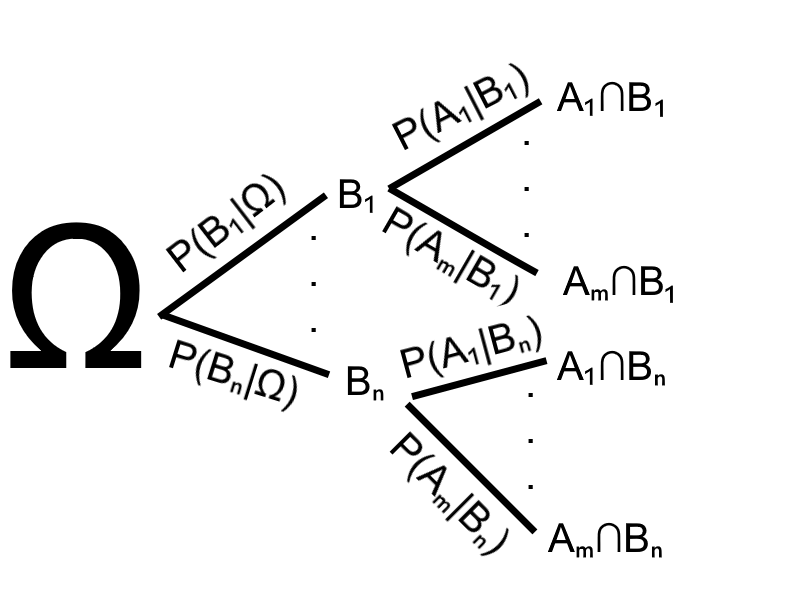
\includegraphics[width=200pt]{tree.png}
		\begin{align*}
			P(A_1\cap B_1)&=P(A_1|B_1)P(B_1)\\
			P(A_m\cap B_1)&=P(A_m|B_1)P(B_1)\\
			P(A_1\cap B_n)&=P(A_1|B_n)P(B_n)\\
			P(A_m\cap B_n)&=P(A_m|B_n)P(B_n)\\\\
			\sum_{i, j=1}^{m, n}P(A_i\cap B_j)&=\sum_{i, j=1}^{m, n}P(A_i|B_j)P(B_j)\\
			&=\sum_{i=1}^m\sum_{j=1}^nP(A_i|B_j)P(B_j)\\
			&=P(\bigcup_{i=1}^mA)\\
			&=P(\Omega)\\
			&=1
		\end{align*}
	\end{myrem}
	
	\begin{myex}{}{}
		\begin{enumerate}
			\item Consider an urn with 2 dice, where $die_1$ has sides (1, 1, 1, 6, 6, 6) and $die_2$ has sides (1, 2, 3, 4, 5, 6). Draw a die at random and roll it. What is $P(``roll\;6")$?
		
			Let $\Omega=\{(1, 1), (1, 6), (2, 1), \dots, (2, 6)\}$, $\mathcal{F}=\mathcal{P}(\Omega)$. Define $P$ as:\\
			\begin{center}
				\begin{tabular}{c|c|c|c|c|c} 
					 $(\omega_1, \omega2)$ & (1, 1) & (1, 6) & (2, 1) & \dots & (2, 6) \\
					 \hline
	$P(\{(\omega_1, \omega_2)\})$ & $\frac{1}{2}\frac{1}{2}=\frac{1}{4}$ & $\frac{1}{2}\frac{1}{2}=\frac{1}{4}$ & $\frac{1}{2}\frac{1}{6}=\frac{1}{12}$ & $\frac{1}{2}\frac{1}{6}=\frac{1}{12}$ & $\frac{1}{2}\frac{1}{6}=\frac{1}{12}$
				\end{tabular}
			\end{center}
			
			Let $A=``Rolling\;6"=\{(\omega_1, \omega_2)\in\Omega : \omega_2=6\}$\\
			$B=``Drawing\;die\;1"=\{(\omega_1, \omega_2)\in\Omega : \omega_1=1\}$
			\begin{align*}
				P(A)&=P(A|B)P(B)+P(A|B^c)P(B^c)\\
				&=\frac{1}{2}\frac{1}{2}+\frac{1}{6}\frac{1}{2}\\
				&=\frac{1}{3}
			\end{align*}
			
			\item Monty Hall problem.\\\\
			Suppose you can choose between 3 doors. Behind one is a car, behind the others are goats. You pick a door, wlog, $door_1$.\\
			The host then, possibly randomly, opens one of the other doors, with a goat behind it. He then gives you a chance to switch to the remaining door. Should you (assuming you want a car more than you want a goat)?\\\\
			Let $\Omega=\{(\omega_1, \omega_2) : \omega_1\in\{1, 2, 3\}, i=1, 2\}$, where $\omega_1$ represents the door containing a car and $\omega_2$ represents the door the host reveals.\\
			Let $\mathcal{F}=\mathcal{P}(\Omega)$\\
			Let $A_i=\{(\omega_1, \omega_2)\in\Omega : \omega_1=i\}, i=1, 2, 3$\\
			$B_j=\{(\omega_1, \omega_2)\in\Omega : \omega_2=j\}, i=2, 3$\\
			
			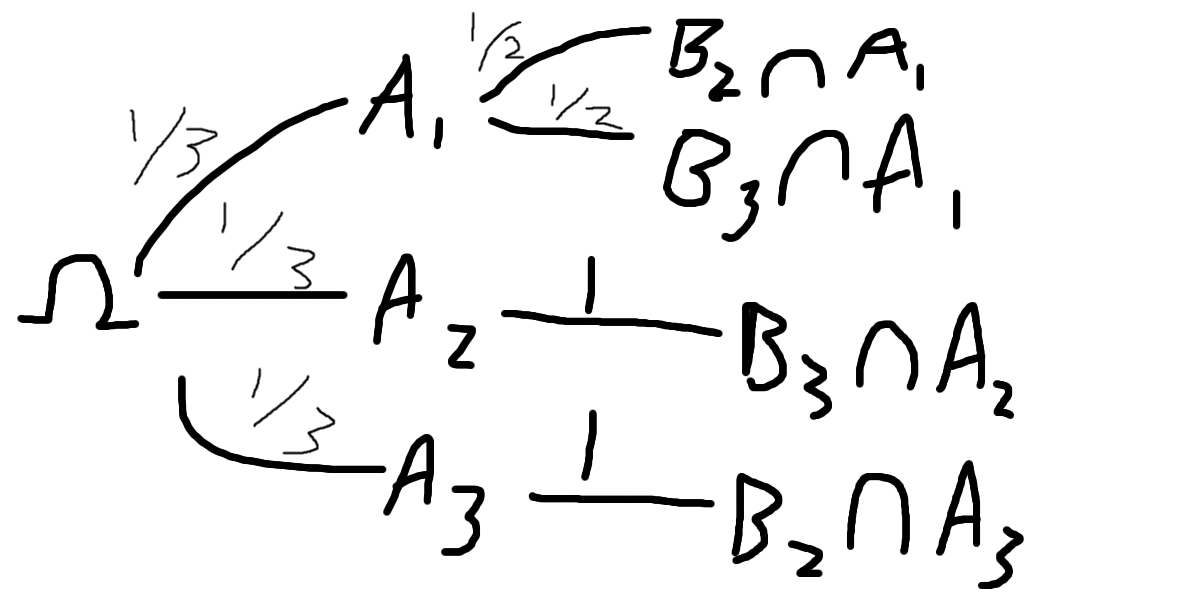
\includegraphics[width=200px]{tree2.png}
			
			\begin{align*}
				\Rightarrow P(A_1\cap B_2) n&=P(B_2|A_1)P(A_1)=\frac{1}{2}\frac{1}{3}=\frac{1}{6}\\
				P(A_1\cap B_3) n&=P(B_3|A_1)P(A_1)=\frac{1}{2}\frac{1}{3}=\frac{1}{6}\\
				P(A_2\cap B_3) n&=P(B_3|A_2)P(A_2)=1\frac{1}{3}=\frac{1}{3}\\
				P(A_3\cap B_2) n&=P(B_2|A_3)P(A_3)=1\frac{1}{3}=\frac{1}{3}\\\\
			\end{align*}
			\[
				\Rightarrow	P(\{(\omega_1, \omega_2)\})=\begin{cases}
					\frac{1}{6} &\mbox{if } (\omega_1, \omega_2)=(1, 2)\\
					\frac{1}{6} &\mbox{if } (\omega_1, \omega_2)=(1, 3)\\
					\frac{1}{3} &\mbox{if } (\omega_1, \omega_2)=(2, 3)\\
					\frac{1}{3} &\mbox{if } (\omega_1, \omega_2)=(3, 2)\\
					0 &\mbox{otherwise}					
			\end{cases}
			\]
			So, $P(\mbox{winning when not switching})=P(\{(\omega_1, \omega_2)\in\Omega : \omega_1=1\})=\frac{1}{6}+\frac{1}{6}=\frac{1}{3}\\
			P(\mbox{winning when switching})=P(\{(2, 3), (3, 2)\})=\frac{1}{3}+\frac{1}{3}=\frac{2}{3}$
			$\therefore$ switching is better.\\
			
			We can also see this from
			\begin{align*}
				P(A_2|B_3)&=\frac{P(A_2\cap B_3)}{P(B_3)}\\
				&=\frac{P(A_2\cap B_3}{P(A_1\cap B_3)+P(A_2\cap B_3)+P(A_3\cap B_3)}\\
				&=\frac{\frac{1}{3}}{\frac{1}{6}+\frac{1}{3}+0}\\
				&=\frac{2}{3}\\
			\end{align*}
			Which also equals $P(A_3|B_2)$ by a similar argument.
		\end{enumerate}
	\end{myex}
	
	\begin{mythm}{Bayes' Theorem}{}
		Let $(\Omega, \mathcal{F}, P)$ be a probability space,\\
		$A\in\mathcal{F}$ such that $P(A)>0$.\\
		Then, $P(B|A)=\frac{P(A|B)P(B)}{P(A)}$ for $A, B\in\mathcal{F}$. Also, if $\{B_i\}_{i\in\mathbb{N}}\subseteq\mathcal{F}$ is a partition of $\Omega$, then
		\begin{align*}
			P(B_i|A)&=\frac{P(A_i|B)P(B_i)}{P(A)}\\
			&=\frac{P(A|B_i)P(B_i)}{\sum_{j=1}^{\infty}P(A|B_j)P(B_j)}
		\end{align*}
		\begin{proof}
			$P(B|A)=\frac{P(B\cap A)}{P(A)}=\frac{P(A\cap B)}{P(A)}=\frac{P(A|B)P(B)}{P(B)}$
		\end{proof}
	\end{mythm}
	
	\begin{myex}{}{}
		A phone sends 0s and 1s (ratio = 3:2) to an antenna. With a certain probability $p\in(0, 1)$, 0s are received wrongly as 1s. With a certain probability $q\in(0, 1)$, 1s are received wrongly as 0s.
		\begin{enumerate}[label=(\alph*)]
			\item Find probability that a 1 is received.
			\item Find probability that a 1 has been sent, given a 1 has been received.
		\end{enumerate}
		\paragraph{Solution.}
		\begin{enumerate}[label=(\alph*)]
			\item Let $\Omega=\{\omega_1, \omega_2) : \omega_i\in\{0, 1\}, i=1, 2\}\\
			\mathcal{F}=\mathcal{P}(\Omega)\\
			S_i=$``i sent"$=\{(i, 0), (i, 1)\}\;i=0, 1\\
			R_i=$``i received"$=\{(0, i), (1, i)\}\;i=0, 1$. Then,
			\begin{align*}
				P(R_1)&=P(R_1|S_0)P(S_0)+P(R_1|S_1)P(S_1)\\
				&=p\frac{3}{5}+(1-q)\frac{2}{5}\\
				&=0.6p+0.4(1-q)
			\end{align*}
			\item
			\begin{align*}
				P(S_1|R_1)&=\frac{P(R_1|S_1)P(S_1)}{P(R_1)}\\
				&=\frac{0.4(1-q)}{0.6p+0.4(1-q)}
			\end{align*}
			From (a).
		\end{enumerate}
	\end{myex}
	
	If $P(A|B)$ does not depend on $B$, then $$P(A\cap B)=P(A|B)P(B)=P(A)P(B)$$
	These events are independent.
	\begin{mydef}{Independence}{}
		Let $(\Omega, \mathcal{F}, P)$ be a probability space. Then
		\begin{enumerate}[label=(\roman*)]
			\item $A_1, A_2\in\mathcal{F}$ are \underline{independent} if $P(A_1\cap A_2)=P(A_1)P(A_2)$.
		\end{enumerate}
	\end{mydef}
\end{document}